%%%%%%%%%%%%%%%%%%%%%%%%%%%%%%%%%%%%%%%%%%%%%%%%%%%%%%%%%%%%%%%%%%%%%%%%%%%%%
%% INÍCIO CAPÍTULO                                                         %%
%%%%%%%%%%%%%%%%%%%%%%%%%%%%%%%%%%%%%%%%%%%%%%%%%%%%%%%%%%%%%%%%%%%%%%%%%%%%%

\chapter{Desenvolvimento}
\label{cap:3:desenvolvimento}

Neste capítulo é apresentada uma breve descrição do \textit{boilerplate} do sistema, destacando os principais aspectos da arquitetura e implementação.

A Seção~\ref{sec:3:estrutura-projeto} apresenta a estrutura do projeto, a partir da instalação e configuração, destacando a organização dos arquivos, utilitários, módulos e suas respectivas responsabilidades. A proposição de uma estrutura bem definida é fundamental para a manutenção e evolução do sistema, além de facilitar o desenvolvimento de novas funcionalidades.

Na Seção~\ref{sec:3:estado-observador}, são detalhados os fundamentos da estrutura de interação com a interface gráfica, que utiliza principalmente dois padrões de projeto: \textit{Observer} e \textit{State}. Esses padrões definem como as interações entre a interface gráfica e os estados de contexto da aplicação são realizadas, garantindo modularidade e eficiência.

A Seção~\ref{sec:3:controller-module} são descritas as camadas de \textit{controller} e \textit{module}, que desempenham, respectivamente, o papel de conectar as ações dos \textit{widgets} e assegurar a propagação dos estados para o restante da aplicação.

A descrição do contexto global de estados pode ser observada na Seção~\ref{sec:3:store}, que apresenta o módulo de gerenciamento de estados, que centraliza as operações relacionadas e fornece uma interface para salvar e restaurar o estado da aplicação. Esse módulo simplifica a integração dos estados com a interface gráfica, fornecendo uma forma eficiente de reutilização da aplicação, ao permitir que o estado seja salvo e restaurado em cada execução.

Na Seção~\ref{sec:3:banco-de-dados} é apresentado o módulo de banco de dados, que fornece uma interface simples para salvar e carregar dados eficientemente. Esse módulo fornece uma camada de abstração para a manipulação de dados, permitindo salvar informações como estados, configurações, resultados, parâmetros de modelos e outros dados relevantes para a aplicação.

Os modelos de pré-processamento, processamento e avaliação são apresentados na Seção~\ref{sec:3:modelos}, destacando as principais características e funcionalidades do gerenciador de modelos. Esses modelos são essenciais para a execução das rotinas de análise de dados, fornecendo interfaces para salvar, carregar e executar modelos treinados.

A interface gráfica criada como exemplo para o \textit{boilerplate} é descrita na Seção~\ref{sec:3:interface-grafica}, destacando as principais funcionalidades e elementos visuais. Essa interface é um exemplo de como os conceitos e padrões de projeto apresentados podem ser aplicados na prática, fornecendo uma base sólida para o desenvolvimento de aplicações mais complexas.

O conjunto de utilitários é descrito na Seção~\ref{sec:3:utils}, que fornece uma série de funções e ferramentas para facilitar o desenvolvimento de aplicações. Esses utilitários incluem funções para auditoria, verificação de código, documentação e internacionalização.

Para rever todos os aspectos do desenvolvimento e uso da aplicação desenvolvida, na Seção~\ref{sec:3:consideracoes-finais} é apresentado um resumo das principais funcionalidades e características do sistema, destacando os principais pontos abordados e sua relevância no contexto geral do trabalho.

% ========================================================================= %

\section{Arquitetura}
\label{sec:3:estrutura-projeto}

Nesta seção, é apresentada a instalação, configuração do projeto e execução, destacando as dependências e ferramentas utilizadas. Em seguida, é descrita a estrutura de arquivos e diretórios do projeto, com ênfase nos principais elementos. Por fim, é apresentada a arquitetura geral do projeto, destacando os principais componentes e suas interações.

\subsection{Instalação e Configuração}
\label{sec:3:install-configure}

Para melhor compreensão da arquitetura do projeto, é importante conhecer as dependências e ferramentas utilizadas. Para auxiliar no entendimento deste capítulo, a instalação e configuração do projeto são descritas nesta Subseção~\ref{sec:3:install-configure}.

\subsubsection{Importação}
\label{subsec:3:importacao}

Para obter acesso ao projeto é possível importar a partir do \textbf{GitHub} por meio do comando \verb|git clone git@github.com:ZauJulio/FeaturesAnalyzer.git| ou baixando o arquivo compactado diretamente do repositório. A \textit{branch} \texttt{test} contém a versão utilizada neste trabalho, que pode ser acessada com o comando \verb|git checkout test|.

\newcommand\urlPyproject{https://github.com/ZauJulio/FeaturesAnalyzer/blob/test/pyproject.toml}
\newcommand\urlRequirements{https://github.com/ZauJulio/FeaturesAnalyzer/blob/test/requirements.txt}

Após a importação, é necessário instalar as dependências do projeto, que estão listadas no arquivo \href{\urlPyproject}{\underline{pyproject.toml}}\footnote{\url{\urlPyproject}} e \href{\urlRequirements}{\underline{requirements.txt}}\footnote{\url{\urlRequirements}}.

\subsubsection{Instalação}
\label{subsec:3:instalacao}

Para instalar as dependências do projeto, é recomendado o uso do \href{https://python-poetry.org/docs/#installing-with-pipx}{\underline{poetry}} com \href{https://github.com/pyenv/pyenv?tab=readme-ov-file#installation}{\underline{pyenv}}, que facilita a gestão de dependências e ambientes virtuais. O \texttt{poetry} utiliza os arquivos \texttt{pyproject.toml} e \texttt{poetry.lock} para registrar as configurações e dependências do projeto, garantindo a reprodutibilidade do ambiente em diferentes sistemas e colaboradores.

Com o \texttt{poetry} instalado, as dependências podem ser instaladas com o comando \verb|make prepare|. Caso o comando \texttt{make} não esteja disponível, é possível instalar de acordo com cada distribuição.

\begin{itemize}
    \item Debian/Raspbian/Ubuntu/Kali: \verb|apt-get install make|
    \item Alpine: \verb| apk add make|
    \item Arch: \verb| Linux pacman -S make|
    \item CentOS: \verb| yum install make|
    \item Fedora: \verb| dnf install make|
    \item Windows: \verb| (WSL2)|
    \item OS X: \verb|brew install make|
\end{itemize}

Caso o \texttt{poetry} não esteja disponível, as dependências podem ser instaladas manualmente com o \texttt{pip}. Para isso, basta executar o comando \verb|pip install -r requirements.txt| na raiz do projeto.

\subsubsection{Configuração}
\label{subsec:3:configuracao}

\newcommand\urlEnv{https://github.com/ZauJulio/FeaturesAnalyzer/blob/test/.env.example}

Além das dependências, o projeto conta com arquivos de configuração na raiz, como o \texttt{.env.example}, \texttt{mkdocs.yml} e \texttt{ruff.toml}, que facilitam o gerenciamento do ambiente. O arquivo \href{\urlEnv}{\underline{.env.example}}\footnote{\url{\urlEnv}} contém variáveis de ambiente que devem ser configuradas conforme as necessidades do projeto em um novo arquivo \texttt{.env}.

\subsubsection{Execução}
\label{subsec:3:execucao}

\newcommand\urlMakefile{https://github.com/ZauJulio/FeaturesAnalyzer/blob/test/Makefile}

Após a instalação e configuração do projeto, a execução pode ser feita de maneira simplificada com o comando \verb|make run|. Além da instalação e execução, o \texttt{Makefile} conta com outros comandos úteis, como \texttt{lint}, \texttt{serve} e \texttt{migrate-deps} para facilitar o desenvolvimento e manutenção do projeto. Para mais informações, consulte o arquivo \href{\urlMakefile}{\underline{Makefile}}\footnote{\url{\urlMakefile}}.

Uma vez que o projeto foi importado, as dependências instaladas e as configurações realizadas, é possível acompanhar o desenvolvimento deste capítulo com a execução do projeto.

\subsection{Estrutura de Arquivos e Diretórios}
\label{subsec:3:estrutura-arquivos}

A descrição da arquitetura inicia-se pela organização da estrutura de arquivos do projeto, destacando os diretórios e arquivos mais relevantes. Esta estrutura foi planejada para garantir a modularidade, clareza e facilidade de manutenção do código. Na Figura~\ref{fig:3:dir-files} é apresentada a estrutura de arquivos e diretórios do projeto, detalhada na Lista~\ref{list:3:estrutura-arquivos}, e na Figura~\ref{fig:3:cd-arch} sua arquitetura geral, que será discutida em detalhes nas próximas seções.

\renewcommand*\DTstylecomment{\rmfamily\small\color{gray}\textsc}

\begin{figure}[h!]
    \dirtree{%
    .1 src.
        .2 assets \DTcomment{Arquivos de recursos do projeto}.
            .3 styles \DTcomment{Estilos globais}.
            .3 icons \DTcomment{Ícones}.
        .2 docs \DTcomment{Documentação usada pelo MkDocs}.
        .2 i18n \DTcomment{Arquivos de internacionalização}.
        .2 src \DTcomment{Código-fonte do projeto}.
            .3 context \DTcomment{Estado global}.
                .4 states/* \DTcomment{Estados com manipuladores}.
                .4 store.py \DTcomment{Gerenciador de contexto}.
            .3 models/* \DTcomment{Modelos do projeto, baseados em FAModel}.
            .3 interfaces \DTcomment{Interfaces do projeto}.
                .4 application.py \DTcomment{Interface global da aplicação}.
                .4 controller.py \DTcomment{Manipulador genérico e conexão de sinais}.
                .4 module.py \DTcomment{Manipulador de sinais de estado raiz}.
                .4 state.py \DTcomment{Estado genérico}.
                .4 widget.py \DTcomment{Widget genérico, estende Gtk.Widget}.
            .3 lib \DTcomment{Bibliotecas do projeto}.
                .4 model\_manager \DTcomment{Gerenciador de modelos}.
                .4 orm \DTcomment{ORM tipado com Pydantic e TinyDB}.
                .4 state\_manager \DTcomment{Gerenciador de estados com Observer}.
                .4 utils \DTcomment{Utilitários genéricos}.
                    .5 bin\_.py \DTcomment{Acesso a modelos binários}.
                    .5 hash.py \DTcomment{Utilitários de hash}.
                    .5 lock.py \DTcomment{Utilitários para multiprocessamento}.
                    .5 logger.py \DTcomment{Logger global}.
                    .5 meta.py \DTcomment{Utilitários de \textit{metaclasses}, como \textit{Singleton}}.
                    .5 time\_.py \DTcomment{Fusos horários, etc.}.
                    .5 types\_.py \DTcomment{Tipos para o gerenciador de estados}.
                    .5 ui.py \DTcomment{Utilitários de interface gráfica}.
                .4 widget.py \DTcomment{Widget genérico, estende Gtk.Widget}.
            .3 sdk \DTcomment{SDKs para outros serviços}.
        .2 .env.example \DTcomment{Exemplo de variáveis de ambiente}.
        .2 Makefile \DTcomment{Makefile com comandos comuns}.
        .2 pyproject.toml \DTcomment{Configuração do projeto Python}.
        .2 requirements.txt \DTcomment{Dependências Python (alternativa ao Poetry)}.
    }
    \caption{Estrutura de Arquivos e Diretórios do Projeto.}
    \centerline{\textbf{Fonte:} O Próprio Autor (2025)}
    \label{fig:3:dir-files}
\end{figure}

\newpage

\subsubsection{Descrição Geral}

A estrutura de arquivos segue boas práticas de organização, com destaque para:

\begin{itemize}\label{list:3:estrutura-arquivos}
    \item \textbf{assets}: Armazena arquivos de recursos visuais, como estilos e ícones.

    \item \textbf{docs}: Contém a documentação do projeto, que pode ser gerada com ferramentas como o \texttt{MkDocs}.

    \item \textbf{i18n}: Centraliza os arquivos de internacionalização, permitindo suporte a múltiplos idiomas.

    \item \textbf{src}: Diretório principal do código-fonte, subdividido em módulos funcionais, como \texttt{context}, \texttt{models} e \texttt{lib}.

    \begin{itemize}
        \item \textbf{context}: Inclui o estado global da aplicação, com os estados e manipuladores associados.

        \item \textbf{models}: Contém os modelos do projeto, baseados na classe \texttt{FAModel}.

        \item \textbf{interfaces}: Define as interfaces do projeto, como \texttt{Application} e \texttt{Controller}.

        \item \textbf{lib}: Agrupa as bibliotecas do projeto, organizadas em subdiretórios, como gerenciadores de modelos e utilitários gerais.
    \end{itemize}

    \item Arquivos de configuração (\texttt{.env.example}, \texttt{Dockerfile}, \texttt{Makefile}, etc.) estão localizados na raiz, facilitando a automação e o gerenciamento do ambiente.
\end{itemize}

\begin{figure}[h!]
    \centerline{\includesvg[width=1\columnwidth]{image/source/cd-arch.svg}}
    \caption{Diagrama Geral de Arquitetura.}
    \centerline{\textbf{Fonte:} O Próprio Autor (2025)}
    \label{fig:3:cd-arch}
\end{figure}

Nesta Seção~\ref{sec:3:estado-observador} é detalhado a implementação do componente base, que fornece a infraestrutura para a interface gráfica e o gerenciamento de estados.

\footnote{Durante o desenvolvimento do sistema, o projeto recebeu o nome provisório de \textit{Features Analyzer} (do inglês, Analisador de Características) (FA). Por essa razão, a sigla \textit{FA} pode ser encontrada em diversos módulos e classes, sendo utilizada para distinguir os componentes do \textit{boilerplate} daqueles específicos da aplicação que o utiliza. Essa abordagem contribui para uma separação clara entre a estrutura base e as personalizações realizadas para cada sistema desenvolvido.}



% ========================================================================= %

\section{Observador e Estado}
\label{sec:3:estado-observador}

A base do \textit{boilerplate} da aplicação é construída com a associação de dois padrões de projeto fundamentais: \textit{Observer} (Observador) e \textit{State} (Estado). Essa seção é ilustrada na Figura~\ref{fig:3:cd-arch} caixa azul, posicionada a direita, com título \textbf{\textit{State}}.

O padrão \textit{Observer} é utilizado para notificar funções de \textit{callback} (funções que executam rotinas específicas utilizadas como parâmetro) quando um determinado contexto é alterado. Já o padrão \textit{State} é empregado para o armazenamento de informações, além de possibilitar a criação de \textit{getters} e \textit{setters} para manipulação eficiente do estado.

Ao associar esses dois padrões a um \textit{Widget}, é possível salvar e manipular o estado de um componente de maneira eficiente, utilizando \textit{handler's} (funções responsáveis por tratar objetos específicos) para gerenciar o estado, e notificações de mudanças por meio de \textit{callback's} fornecidos ao \textit{Observer}. O diagrama de classe ilustrado na Figura~\ref{fig:3:cd-state-observer} demonstra a relação entre as implementações dos padrões de projeto \textit{Observer} e \textit{State}.

\begin{figure}[h!]
    \centerline{\includesvg[width=1\columnwidth]{image/source/cd-state-observer.svg}}
    \caption{Diagrama de classe dos padrões Estado e Observador.}
    \centerline{\textbf{Fonte:} O Próprio Autor (2025)}
    \label{fig:3:cd-state-observer}
\end{figure}

A implementação desses padrões de projeto estende-se ao domínio do problema do sistema. Nesse contexto, o estado de um objeto pode assumir dois valores distintos simultaneamente: estado rastreado e estado não rastreado.

O estado rastreado é utilizado para armazenar o contexto concreto do objeto; no entanto, assim que ocorre uma alteração, ele se torna um estado não rastreado, pois as mudanças ainda não foram propagadas para as funções observadoras. Para fins de simplicidade, além das abstrações, os estados são dois dicionários, um para o estado rastreado e outro para o estado não rastreado.

O principal objetivo dessa abordagem é evitar a propagação desnecessária de mudanças no estado. Isso é particularmente útil em situações onde o estado do objeto pode ser alterado várias vezes em um curto intervalo de tempo, como durante a interação do usuário com a interface gráfica ao ajustar os parâmetros de um modelo.

Por exemplo, na implementação desenvolvida, um simples botão de salvar pode ser usado para realizar um \textit{commit} do estado, definindo-o como rastreado e propagando as alterações para o restante do sistema.

Nas subseções seguintes, são apresentados os detalhes da implementação dos padrões de projeto \textit{Observer} e \textit{State}, bem como sua utilização para viabilizar a interação eficiente entre a interface gráfica e o módulo de controle.

%%%%%%%%%%%%%%%%%%%%%%%%%%%%%%%%%%%%%%%%%%%%%%%%
\subsection{Observador}

Na implementação do padrão \textit{Observer}, a classe abstrata \texttt{Observer} é responsável por definir a interface de notificação de mudanças de estado. Essa classe é estendida pela classe \texttt{State}, que armazena o estado do objeto observado e notifica os \textit{handlers} de mudança de estado.

O diagrama da classe \texttt{Observer} é apresentado na Figura~\ref{fig:3:cd-state-observer}. No diagrama, os atributos protegidos são identificados pelo símbolo \texttt{\#}, indicando que não podem ser acessados diretamente. As operações públicas, acessíveis por qualquer classe que herde ou instancie \textit{Observer}, são indicadas com \texttt{+}, enquanto as operações privadas, restritas à própria classe, começam com \texttt{-}. Abaixo, são descritos os atributos e operações da classe \texttt{Observer}.

\subsubsection{Atributos}

Todos os atributos da classe \texttt{Observer} são protegidos, garantindo que não sejam acessados diretamente por outras classes. Seus principais atributos incluem:

\begin{itemize}
    \item \texttt{\_status}: Indica o estado atual do objeto observado. Os estados possíveis são:
    \begin{itemize}
        \item \texttt{idle}: O objeto não está em uso por nenhuma operação.
        \item \texttt{committing}: O objeto está sendo atualizado.
        \item \texttt{error}: Ocorreu um erro durante a atualização.
    \end{itemize}
    \item \texttt{\_tracked}: Define se o estado do objeto está rastreado (\texttt{True}) ou não (\texttt{False}), ou seja, não houve alterações desde o último \texttt{commit()}.
    \item \texttt{\_keys}: Armazena as chaves de notificação de mudanças, representando os nomes dos atributos do objeto observado.
    \item \texttt{\_subscribers}: Um objeto que lista os \textit{handlers} que serão notificados sobre mudanças nos atributos observados, conforme as chaves definidas em \texttt{\_keys}.
    \item \texttt{\_root\_subscribers}: Contém \textit{handlers} associados às mudanças de contexto do objeto observado, utilizando as seguintes chaves:
    \begin{itemize}
        \item \texttt{on\_untrack}: Notifica quando o estado deixa de ser rastreado.
        \item \texttt{on\_commit}: Notifica quando o estado é rastreado por meio de um \textit{commit()}.
    \end{itemize}
\end{itemize}

\subsubsection{Operações}

As operações da classe \texttt{Observer} estão organizadas em públicas, protegidas e privadas, conforme descrito abaixo:

\paragraph{Operações públicas:}
\begin{itemize}
    \item \texttt{\_\_init\_\_}: Inicializa os atributos da classe. Recebe como parâmetro \texttt{annotations}, uma lista de chaves de notificação de mudanças (\texttt{subscriber keys}).
    \item \texttt{status}: Retorna o estado atual do objeto observado. Acessado como propriedade (\texttt{property}) e somente leitura.
    \item \texttt{tracked}: Retorna se o estado está sendo rastreado. Propriedade somente leitura, assim como \texttt{status}.
    \item \texttt{untrack}: Define \texttt{\_tracked} como \texttt{False} e notifica \texttt{\_root\_subscribers} com a chave \texttt{on\_untrack}.
    \item \texttt{track}: Define \texttt{\_tracked} como \texttt{True} e ajusta o estado para \texttt{idle}.
    \item \texttt{on\_change}: Adiciona um \textit{handler} de notificação. Recebe como parâmetros:
    \begin{itemize}
        \item \texttt{key}: A chave do atributo observado ou de \texttt{\_root\_subscribers}.
        \item \texttt{handler}: Função de \textit{callback} que recebe os valores antigo e novo do estado.
    \end{itemize}
    \item \texttt{commit}: Atualiza todo valor não rastreado, ou alterado, para o objeto rastreado. Notifica \texttt{\_root\_subscribers} com a chave \texttt{on\_commit} e, para cada atributo alterado, notifica os \texttt{\_subscribers} correspondentes.

    \hfill \break

    Por exemplo, um objeto observado qualquer \verb|{ a : 1 }|, possui duas instancias, uma rastreada e outra não rastreada. Uma vez que o atributo \texttt{a} seja alterado para \texttt{2}, os \textit{handlers} de \texttt{a} são notificados, ou seja, as funções de \textit{callback} associadas a chave \texttt{a} são executadas. As funções recebem os valores antigo e novo do estado, \verb|{ a : 1 }| e \verb|{ a : 2 }| respectivamente, permitindo a execução de lógicas específicas para cada atributo.

    Para rastrear a mudança de estado, o método \texttt{commit} sincroniza o estado rastreado com o valor concreto do objeto, notificando os \texttt{\_subscribers} de \texttt{a} e os \texttt{\_root\_subscribers} de \texttt{on\_commit}. Ao realizar um \texttt{commit}, o estado rastreado é atualizado com o valor do estado não rastreado, logo, o atributo \texttt{a} do objeto rastreado passa a ser \texttt{2}.
\end{itemize}

\paragraph{Operações privadas:}
\begin{itemize}
    \item \texttt{\_\_on\_commit}: Define o estado como \texttt{committing} e notifica \texttt{\_root\_subscribers} com a chave \texttt{on\_commit} durante o gerenciamento de contexto com a cláusula \texttt{with}. Ao final da operação, define o estado como \texttt{idle} através de \texttt{track()}.
\end{itemize}

\paragraph{Operações protegidas:}
\begin{itemize}
    \item \texttt{\_notify}: Notifica \texttt{\_subscribers} e \texttt{\_root\_subscribers} sobre mudanças no estado.
    \item \texttt{\_validate\_keys}: Valida as chaves de notificação recebidas.
    \item \texttt{\_get\_tracked}, \texttt{\_get\_untracked}, \texttt{\_track\_changes}: Métodos abstratos que devem ser implementados para rastrear mudanças de estado.
    \begin{itemize}
        \item \texttt{\_get\_tracked}: Retorna o estado rastreado do objeto observado.
        \item \texttt{\_get\_untracked}: Retorna o estado não rastreado do objeto observado.
        \item \texttt{\_track\_changes}: Sincroniza o estado rastreado com o valor concreto do objeto. Recebe como parâmetro o valor do estado não rastreado e a chave do atributo alterado.
    \end{itemize}
\end{itemize}

A nomenclatura adotada com \texttt{\_} e \texttt{\_\_} indica que os atributos ou métodos são protegidos, ou privados, respectivamente, seguindo as convenções do Python. Embora seja possível acessar diretamente tais elementos, a prática desaconselha esse uso, contribuindo para uma melhor manutenção do código.

\subsubsection{Exemplo de Implementação}

Como exemplo, uma classe pode herdar de \texttt{Observer} e implementar os métodos abstratos \texttt{\_get\_tracked}, \texttt{\_get\_untracked} e \texttt{\_track\_changes}. Essa classe gerencia dois atributos: \texttt{t\_state} (estado rastreado) e \texttt{ut\_state} (estado não rastreado), que possuem as mesmas chaves, como \texttt{a} e \texttt{b}.

Uma vez que um atributo é alterado e o método \texttt{untrack} é chamado, o estado de \_tracked é alterado para falso e os \texttt{\_root\_subscribers} são notificados com a chave \texttt{on\_untrack}. Quando o método \texttt{commit} é chamado, o estado de \texttt{\_tracked} é alterado para verdadeiro e os \texttt{\_root\_subscribers} são notificados com a chave \texttt{on\_commit}. Além disso, os \texttt{\_subscribers} são notificados com a chave correspondente ao atributo que passou por alteração.

A classe \texttt{State}, que herda de \texttt{Observer}, foi criada para evitar duplicação de código, implementando os métodos abstratos necessários para rastrear mudanças de estado de forma automática e eficiente.

%%%%%%%%%%%%%%%%%%%%%%%%%%%%%%%%%%%%%%%%%%%%%%%%
\subsection{Estado}

A classe \texttt{State} é responsável por armazenar o estado de um objeto e, por meio da herança da classe \texttt{Observer}, notificar \textit{handlers} sobre mudanças no estado. Além de herdar os atributos e métodos da classe \texttt{Observer}, a classe \texttt{State} implementa os métodos abstratos \texttt{\_get\_tracked}, \texttt{\_get\_untracked} e \texttt{\_track\_changes}, permitindo a automação no rastreamento e propagação de mudanças no estado.

O objetivo principal da classe \texttt{State} é simplificar a manipulação de objetos com estados rastreáveis, permitindo que os atributos do estado e os manipuladores associados sejam definidos diretamente na classe derivada. Além disso, ela oferece funcionalidades adicionais para gerenciar, serializar e restaurar estados, otimizando sua integração em sistemas dinâmicos.

\subsubsection{Atributos}

\begin{itemize}
    \item \texttt{\_state}: Um dicionário que armazena o estado rastreado do objeto observado. É inicializado com os valores fornecidos no momento da criação da classe através das anotações de tipo e dos valores iniciais passados como parâmetro.
    \item \texttt{\_backup}: Uma cópia temporária do estado rastreado, utilizada para preservar o estado antes de modificações, geralmente em operações envolvendo gerenciamento de contexto.
\end{itemize}

\subsubsection{Operações}

As operações públicas da classe \texttt{State} incluem:

\begin{itemize}
    \item \texttt{\_\_init\_\_}: Inicializa o estado rastreado do objeto com os valores fornecidos por parâmetro em um dicionário \textit{State}.
    \item \texttt{\_\_getitem\_\_}, \texttt{\_\_setattr\_\_}, \texttt{\_\_enter\_\_}, \texttt{\_\_exit\_\_}, \texttt{serialize}, \texttt{reset}, \texttt{load}: Métodos especiais do Python que permitem acessar, atualizar e gerenciar o contexto de execução, respectivamente.
    \begin{itemize}
        \item \texttt{\_\_getitem\_\_}: Permite acessar os atributos do estado como itens de um dicionário, utilizando a notação \texttt{state[key]}. Logo, o estado não rastreado é armazenado como atributo da classe que herdou de \texttt{State}, e os rastreados de \texttt{\_state}.
        \item \texttt{\_\_setattr\_\_}: Atualiza o valor de um atributo no estado não rastreado e dispara os manipuladores de notificação de mudança através da \textit{key} \texttt{on\_untrack}.
        \item \texttt{\_\_enter\_\_}: Inicia o gerenciamento de contexto, armazenando uma cópia do estado atual em \texttt{\_backup}.
        \item \texttt{\_\_exit\_\_}: Finaliza o gerenciamento de contexto, restaurando o estado a partir de \texttt{\_backup} em caso de erro.
    \end{itemize}
    \item \texttt{serialize}: Retorna uma representação serializável do estado atual, ideal para armazenamento ou transmissão.
    \item \texttt{reset}: Restaura o estado rastreado para os valores padrão conforme o tipo, como \texttt{0} para inteiros e \texttt{``''} para strings.
    \item \texttt{load}: Atualiza o estado rastreado com os valores fornecidos no parâmetro dicionário \texttt{value}. Especialmente útil para restaurar estados salvos anteriormente.
\end{itemize}

As operações protegidas da classe \texttt{State} incluem:

\begin{itemize}
    \item \texttt{\_get\_untracked}: Retorna uma instância do estado não rastreado, útil para inspeção sem disparar notificações.
    \item \texttt{\_get\_tracked}: Retorna o estado rastreado atual.
    \item \texttt{\_track\_changes}: Realiza o rastreamento de mudanças em um atributo específico do estado, recebe como parâmetros a chave do atributo e o valor a ser atualizado.
    \item \texttt{\_copy}: Retorna uma cópia de um estado fornecido como parâmetro ou de dicionário como parâmetro (\texttt{cls} or \texttt{obj}).
\end{itemize}

\subsubsection{Uso Prático}

A classe \texttt{State} oferece uma abordagem eficiente para gerenciar estados, integrando rastreamento automático de mudanças com notificação de \textit{handlers}. Esse modelo é especialmente útil em sistemas que dependem de estados compartilhados ou precisam sincronizar alterações em diferentes componentes, como interfaces gráficas ou sistemas distribuídos.

Uma das vantagens dessa classe é a possibilidade de agrupar estados em objetos compostos, facilitando a organização e manutenção de sistemas complexos. Por exemplo, em um sistema com módulos distintos — como importação de dados, pré-processamento e treinamento de modelos — os estados de cada módulo podem ser encapsulados em um dicionário \texttt{Context} ou \texttt{Store}. Isso permite que cada módulo gerencie seu próprio estado de forma independente, evitando interferências entre eles e simplificando a manipulação global, através da centralização dos estados.

Embora seja tecnicamente viável compor estados aninhados (ou "estados de estados"), essa prática não é recomendada. Essa abordagem pode introduzir complexidade desnecessária e problemas de sincronização. Em vez disso, estados relacionados devem ser agrupados em um único objeto, promovendo uma interação mais simples e garantindo a consistência dos dados.

Uma recomendação importante é centralizar no domínio de cada estado os \textit{handlers} que gerenciem mudanças específicas. Por exemplo, em um estado responsável por carregar um arquivo, o \textit{handler} associado pode receber o \textit{path} do arquivo e, após um \texttt{commit}, executar a lógica necessária para carregar o arquivo e atualizar um gráfico ou interface de usuário. Para manter a organização e clareza, é sugerido que cada \textit{handler} seja implementado como um método estático da classe derivada de \texttt{State}, seguindo uma convenção de nomenclatura padrão \verb|handle_{id_seq}_{name}|.

Nesta convenção, \texttt{id\_seq} é um número sequencial único que identifica o \textit{handler}, e \texttt{name} é uma descrição clara da função do \textit{handler}. Por exemplo, um \textit{handler} responsável por carregar arquivos poderia ser nomeado como \texttt{handle\_001\_load\_file}. Essa nomenclatura também evita conflitos de nomes, entre estados e com a própria classe \texttt{State}.

Essa abordagem promove consistência, organização e facilita a manutenção de sistemas complexos que utilizam a classe \textit{State}. A seguir é apresentado um exemplo simples e prático do fluxo de interação entre um \textit{Widget} e um estado gerenciado pela classe \texttt{State}.

\footnote{Utiliza-se a convenção \texttt{id\_seq} para identificar a ordem que o \textit{handler} deve ser executado, e \texttt{name} para descrever a função do \textit{handler}. Embora a nomenclatura seja opcional, ela promove a organização e facilita a manutenção de sistemas complexos, além de evitar conflitos de nomes entre estados, \textit{handlers} e a própria classe \texttt{State}.}

\subsubsection{Widgets e Elementos Visuais}

A biblioteca \texttt{GTK} é utilizada para a construção de interfaces gráficas, permitindo a criação de \textit{widgets} (elementos visuais) personalizados e facilitando a interação com o usuário. A classe \texttt{Widget} encapsula os elementos visuais e manipula as interações, utilizando a classe \texttt{State} para monitorar e notificar as mudanças de estado.

A comunicação entre o \texttt{Widget} e o estado ocorre via \textit{handlers} associados a eventos específicos, como cliques em botões ou alterações de valor. Esses \textit{handlers} são definidos em uma classe derivada de \texttt{State} e acionados pelo \texttt{Widget} em resposta a eventos do usuário. Os \textit{widgets} notificam mudanças ou ações por meio de \textit{signals} do \texttt{GTK}, os quais são conectados aos \textit{handlers} correspondentes. Abaixo, são apresentados alguns exemplos de \textit{widgets} e seus respectivos \textit{signals}:

\begin{itemize}
    \item \texttt{Button}: \texttt{clicked} - Notifica quando o botão é clicado.
    \item \texttt{Entry}: \texttt{changed} - Notifica quando o texto é alterado.
    \item \texttt{ComboBox}: \texttt{changed} - Notifica quando o item selecionado é alterado.
    \item \texttt{CheckButton}: \texttt{toggled} - Notifica quando o botão é alternado.
\end{itemize}

Quando o usuário interage com um \texttt{Widget}, o \textit{signal} correspondente é acionado, invocando o \textit{handler} associado. Por exemplo:

\begin{center}
    \begin{lstlisting}[language=Python, caption=Exemplo da conexão do \textit{signal} \texttt{clicked} de um \textit{Widget} e um \textit{handler}., label=lst:3:widget-handler]
    button.connect("clicked", self.on_button_clicked)
    
    def on_button_clicked(self, widget):
        self.state.handle_001_plot_data()
        self.state.commit()
    \end{lstlisting}
    \centerline{\textbf{Fonte:} O Próprio Autor (2025)}
\end{center}

No código~\ref{lst:3:widget-handler}, o \textit{handler} \texttt{handle\_001\_plot\_data} é executado quando o botão é clicado, realizando a lógica necessária para a plotagem dos dados. Após a execução do \textit{handler}, o estado é atualizado através do método \texttt{commit}, propagando as mudanças para os \textit{handlers} associados. Como o \textit{handler} está inserido no domínio do estado, ele pode acessar informações não rastreadas diretamente com o método \texttt{get\_untracked()} antes da execução do método \texttt{commit()}.

\subsubsection{Exemplo de Interação Widget-Estado}

O fluxograma da interação entre um \texttt{Widget} e um estado gerenciado pela classe \texttt{State} é ilustrado na Figura~\ref{fig:3:cd-state-flowchart}. Neste exemplo, adicionamos uma camada intermediária, o \texttt{Controller}, que gerencia a interação entre o \texttt{Widget} e o estado. O \texttt{Controller} é responsável por conectar os sinais do \texttt{Widget} aos \texttt{setters} do estado, garantindo a correta propagação das mudanças de estado. O \texttt{Controller} também pode conter lógica adicional, como validação de entrada ou formatação de dados, antes de atualizar o estado. A seguir, são descritos os passos do diagrama de sequência.

\begin{figure}[h!]
    \centerline{\includesvg[width=0.7\columnwidth]{image/source/cd-state-flowchart.svg}}
    \caption{Diagrama de sequência de interação \textit{Widget}-Estado.}
    \centerline{\textbf{Fonte:} O Próprio Autor (2025)}
    \label{fig:3:cd-state-flowchart}
\end{figure}

\begin{itemize}
    \item O \textit{signal} de um botão é conectado a um \textit{handler} no \texttt{Controller}.

    \item O \texttt{Controller} assina o estado para receber notificações, \texttt{state.on\_change("on\_untrack", self.on\_untrack)} e \texttt{state.on\_change("on\_commit", self.on\_commit)}.

    \begin{itemize}
        \item \texttt{on\_untrack}: Adiciona um botão de aplicar alterações à interface do usuário.
        \item \texttt{on\_commit}: Atualiza a interface do usuário com o novo estado e oculta o botão de aplicar.
    \end{itemize}

    \item O usuário interage com o \texttt{Widget}, acionando o \textit{signal} \textit{"clicked"}.

    \item O \texttt{Controller} executa a lógica necessária, como validação de entrada ou formatação de dados; após isso, define o valor no estado por meio de um \textit{setter} simples, como \texttt{state.value = value}.

    \item O \texttt{State} notifica os \textit{handlers} associados à chave correspondente, como \texttt{on\_value\_change} e \texttt{on\_untrack}.

    \item O \textit{handler} de \textit{on\_untrack} associado ao \texttt{Controller} executa a lógica necessária, e adiciona a interface do usuário um botão para aplicar as alterações.

    \item O novo botão tem o \textit{signal} conectado a um \textit{handler} no \texttt{Controller}, que executa a chamada para \texttt{state.commit()}.

    \item O usuário interage com o novo \texttt{Widget} do botão, acionando o \textit{signal} \textit{"clicked"}.

    \item O \texttt{Controller} executa a chamada para \texttt{state.commit()}.

    \item O \texttt{State} notifica os \textit{handlers} associados à chave correspondente, como \texttt{on\_commit}.

    \item O \texttt{Controller} executa a lógica necessária, como atualizar a interface do usuário com o novo estado e ocultar o botão de aplicar, já que o estado foi rastreado.
\end{itemize}

Nesta arquitetura o \texttt{Controller} atua como um intermediário entre o \texttt{Widget} e o estado, gerenciando a interação entre eles e garantindo a correta propagação das mudanças de estado. Essa abordagem promove a separação de responsabilidades e facilita a manutenção e evolução do sistema, tornando-o mais modular e flexível.

A camada de \texttt{Widget} é responsável pela interação com o usuário, definindo os elementos visuais, enquanto o \texttt{Controller} gerencia a lógica de execução e a comunicação com o estado. Desta forma, a lógica de validação, formatação e atualização de dados é centralizada no \texttt{Controller}, simplificando a implementação e garantindo a consistência dos dados.

Além da camada de \texttt{Controller}, podemos adicionar uma camada de \texttt{Module} para gerenciar alterações globais no estado, como aquelas notificadas pelas chaves \texttt{on\_untrack} e \texttt{on\_commit}. Na Seção~\ref{sec:3:controller-module} são apresentados os detalhes da implementação do módulo de controle e sua integração com a interface gráfica.


% ========================================================================= %

\section{Controller e Module}
\label{sec:3:controller-module}

A camada de \texttt{Controller} e \texttt{Module} desempenha o papel de separar as responsabilidades na propagação e manipulação dos estados, garantindo a consistência, manutenibilidade e escalabilidade do sistema. Na seção atual é apresentado o conteúdo previamente ilustrado na Figura~\ref{fig:3:cd-arch}, caixa do meio em vermelho, com título \textbf{\textit{Base Component}}.

O \texttt{Controller} é responsável por gerenciar as ações dos \textit{Widgets}, enquanto o \textit{Module} lida com as mudanças de estado desencadeadas por essas ações no escopo do domínio de cada componente. A seguir, na Figura ~\ref{fig:3:cd-controller-module} é apresentado o diagrama de classes do \texttt{Controller} e \texttt{Module}.

\begin{figure}[h!]
    \centerline{\includesvg[width=1\columnwidth]{image/source/cd-controller-module.svg}}
    \caption{Diagrama de classe \textit{Controller}-\textit{Module}.}
    \centerline{\textbf{Fonte:} O Próprio Autor (2025)}
    \label{fig:3:cd-controller-module}
\end{figure}

\newpage

\subsection{Controller}
\label{subsec:3:controller}

Nas subseções a seguir é apresentada a implementação da classe \texttt{Controller}.

\subsubsection{Atributos}
\label{subsec:3.3.1:attributes}

\begin{itemize}
    \item \texttt{state}: Uma instância de \texttt{FAState} que armazena o estado do objeto observado. É utilizado para registrar os valores dos widgets e notificar os \textit{handlers} de mudanças.

    \item \texttt{widget}: Uma instância de \texttt{Gtk.Widget} que representa o elemento visual associado ao \texttt{Controller}. É utilizado para conectar os sinais do widget aos \textit{handlers} do \texttt{Controller}. Tipicamente pode ser um único botão ou um contêiner com vários elementos.
\end{itemize}

\subsubsection{Operações}
\label{subsec:3.3.2:operations}

As operações da classe \texttt{Controller} incluem:

\begin{itemize}
    \item \texttt{\_\_init\_\_}: Inicializa o \texttt{Controller} com uma instância de \texttt{State}, um \texttt{widget} associado é instanciado como parâmetro.

    \item \texttt{show}: Exibe o(s) \texttt{widget(s)} associado(s) ao \texttt{Controller}.

    \item \texttt{hide}: Oculta o(s) \texttt{widget(s)} associado(s) ao \texttt{Controller}.

    \item \texttt{\_connect\_signals}, \texttt{reset} e \texttt{load}: Métodos abstratos protegidos que devem ser implementados na classe derivada de \texttt{Controller}.

    \begin{itemize}
        \item \texttt{\_connect\_signals}: Conecta os sinais do \texttt{widget} aos \textit{handlers} do \texttt{Controller}.

        \item \texttt{reset}: Restaura o estado do \texttt{widget} para os valores padrão.

        \item \texttt{load}: Atualiza o estado do \texttt{widget} com os valores fornecidos no parâmetro \texttt{value} do tipo \texttt{State}.
    \end{itemize}
\end{itemize}

No código~\ref{lst:3:controller} é apresentado um exemplo prático de implementação do \texttt{Controller} para um componente que controla os parâmetros de um modelo utilizando KMeans.

\hfill \break

\begin{center}
    \lstinputlisting[basicstyle=\tiny, firstnumber=8, language=Python, firstline=8, lastline=24, caption={Exemplo de implementação do Controller.}, label={lst:3:controller}, label={lst:3:controller}]{code/controller.py}
    \centerline{\textbf{Fonte:} O Próprio Autor (2025)}
\end{center}

\hfill \break

Na linha \texttt{8}, é possível observar um decorador sobre a classe \texttt{@FAMetaCheckController}, responsável por verificar se os atributos necessários e seus respectivos tipos estão presentes na classe derivada. Esse decorador é uma abstração que simplifica a criação de novos \textit{Controller's}, assegurando a consistência e integridade da implementação.

\newcommand\urlSidebarItem{https://github.com/ZauJulio/FeaturesAnalyzer/blob/test/src/ui/components/shared/sidebar_item/widget.py}

A linha \texttt{10} define a classe \texttt{KMeansSolverController}, que herda de \texttt{Controller} com o tipo \texttt{KMeansSolverState}. Essa sintaxe especifica que o atributo \texttt{State} é uma instância de \texttt{KMeansSolverState}. Além disso, na linha \texttt{13}, é definida a instância do \texttt{widget} associado ao \texttt{Controller}, que pode ser encontrado no \href{\urlSidebarItem}{\underline{arquivo}}\footnote{\url{\urlSidebarItem}}.

No método \texttt{\_\_init\_\_} de \texttt{KMeansSolverController}, iniciado na linha \texttt{15}, observa-se a chamada do método \texttt{\_connect\_signals}, responsável por conectar os sinais do \texttt{widget} aos \textit{handlers} do \texttt{Controller}. Já na linha \texttt{21}, o método \texttt{load} é invocado para atualizar o estado do \texttt{widget} com os valores fornecidos no parâmetro \texttt{State}, o qual é do tipo \texttt{KMeansSolverState}. Por fim, caso algum valor tenha sido enviado através do parâmetro \texttt{State}, o widget adiciona, na linha \texttt{24}, um botão para aplicar as alterações.

O exemplo apresentado demonstra a implementação de um \texttt{Controller}, evidenciando a simplicidade e a organização do código, que contribuem para a manutenção e evolução do sistema. Abstrações como o decorador \texttt{@FAMetaCheckController} e a classe \texttt{Controller} promovem consistência e robustez na implementação, assegurando a qualidade do sistema na totalidade.

\subsection{Module}

A seguir é apresentado o diagrama de classes do \texttt{Module} na Figura~\ref{fig:3:cd-controller-module}. O \texttt{Module} é responsável por gerenciar as mudanças de estado no escopo do domínio de cada componente, assegurando a consistência e a propagação das alterações para o restante do sistema. Essa abstração encapsula a lógica global do estado por meio de uma instância de \texttt{app}, permitindo interação com outros módulos e componentes.

\subsubsection{Atributos}

A classe \texttt{Module} possui os seguintes atributos:

\begin{itemize}
    \item \texttt{name}: Uma string que representa o nome do módulo. É utilizada para identificar o módulo de forma única.

    \item \texttt{app}: Uma instância de \texttt{App} que representa a aplicação principal. Esse atributo permite a interação com outros módulos e componentes, mas deve ser utilizado com cuidado para evitar acoplamento excessivo.

    \item \texttt{State}: Uma instância de \texttt{State} que armazena o estado do objeto observado. Esse estado é utilizado para observar mudanças notificadas pelas chaves \texttt{on\_untrack} e \texttt{on\_commit}.
\end{itemize}

\subsubsection{Operações}

As operações da classe \texttt{Module} incluem:

\begin{itemize}
    \item \texttt{\_\_init\_\_}: Inicializa o \texttt{Module} com uma instância de \texttt{app} e um \texttt{controller} associado ao tipo de estado especificado. A instância de \texttt{app} representa a aplicação principal, possibilitando a interação com outros módulos e componentes.

    \item \texttt{show}: Exibe o(s) \texttt{widget(s)} associado(s) ao \texttt{Controller}.

    \item \texttt{hide}: Oculta o(s) \texttt{widget(s)} associado(s) ao \texttt{Controller}.

    \item \texttt{reset}: Restaura os valores do \texttt{widget} e do estado para os valores padrão. Após a execução, o estado é automaticamente rastreado.

    \item \texttt{load}: Atualiza os valores do \texttt{widget} e do estado com os dados fornecidos no parâmetro \texttt{value} do tipo \texttt{State}. Assim como no método \texttt{reset}, o estado é rastreado após a execução.

    \item \texttt{subscribe}: Adiciona um \textit{handler} para notificações de mudanças no estado das chaves \texttt{on\_untrack} e \texttt{on\_commit}. O \textit{handler} é uma função de \textit{callback} que recebe os valores antigo e novo do estado. Para centralizar a lógica do domínio, os \texttt{handlers} são declarados como métodos estáticos da classe derivada de \texttt{State}.
\end{itemize}

Com base no \texttt{Controller} apresentado na Seção~\ref{subsec:3:controller}, é apresentado a seguir a implementação do \texttt{Module} correspondente, Código~\ref{lst:3:module}.

\begin{center}
    \lstinputlisting[basicstyle=\tiny, numbers=right, firstnumber=11, language=Python, firstline=11, lastline=37, caption={Exemplo de implementação do Module.}, label={lst:3:module}]{code/module.py}
    \centerline{\textbf{Fonte:} O Próprio Autor (2025)}
\end{center}


\hfill \break

Na linha \texttt{11}, observa-se novamente o decorador \texttt{@FAMetaCheckModule}, que verifica se os atributos necessários e seus respectivos tipos estão presentes na classe derivada. A declaração da classe na linha \texttt{12} define a \texttt{KMeansSolverModule}, que herda de \texttt{Module} com os tipos \texttt{KMeansSolverController} e \texttt{KMeansSolverState}. Essa abordagem permite manter referências para ambos os tipos de estado e \texttt{controller} associados ao módulo.

Além disso, na linha \texttt{16}, a tipagem de \texttt{app} é feita entre aspas devido à necessidade de definição explícita para verificação do código. A classe \texttt{FeaturesAnalyzer}, por ser uma das primeiras a ser instanciadas, é importada apenas para verificação de tipo, evitando dependências cíclicas.

Na linha \texttt{19}, o \texttt{Module} é inicializado com uma instância de \texttt{app} e um \texttt{controller} correspondente ao tipo de estado associado. A inicialização da classe base é garantida pela chamada \texttt{super().\_\_init\_\_()}. Como a classe base já invoca o método \texttt{subscribe} na linha \texttt{22}, não é necessário chamá-lo explicitamente.

Por fim, destaca-se o exemplo de conexão entre as atualizações de estado global pelas chaves \texttt{on\_untrack} e \texttt{on\_commit}, utilizando gerenciadores de contexto no método \texttt{subscribe}, localizado na linha \texttt{22}. Por meio da cláusula \texttt{with}, o uso de gerenciadores de contexto assegura que as atualizações de estado sejam realizadas de forma segura e consistente, mitigando problemas de inconsistência causados por falhas nos \texttt{handlers}. Caso ocorra algum erro, o estado é restaurado utilizando o atributo \texttt{\_backup}. A implementação desse gerenciador de contexto encontra-se nos métodos \texttt{\_\_enter\_\_} e \texttt{\_\_exit\_\_} da classe \texttt{State}.

No contexto mencionado, a chave \texttt{on\_untrack} conecta-se ao \texttt{handler} \texttt{on\_module\_change} do widget, que atualiza a interface do usuário adicionando um botão para aplicar alterações por meio do método \texttt{state.commit()}. Esse botão, por sua vez, aciona o método \texttt{commit()} através de \texttt{handle\_status()} do widget. A implementação detalhada desse método pode ser encontrada no arquivo \href{https://github.com/ZauJulio/FeaturesAnalyzer/blob/test/src/ui/components/shared/sidebar_item/widget.py}{\underline{src/ui/components/shared/sidebar\_item/widget.py}}~\ref{note:sidebar} mencionado anteriormente.

Já a chave \texttt{on\_commit}, associada ao \texttt{handler} \texttt{handle\_001\_on\_params\_update}, aplica as alterações de parâmetros ao modelo após o acionamento do botão. Adicionalmente, essa mesma chave conecta-se ao método \texttt{dump} da classe \texttt{Store}, que consolida todos os estados da aplicação em um único contexto. Na Seção~\ref{sec:3:store}, serão apresentados mais detalhes sobre a classe \texttt{Store}. Por fim, na Figura~\ref{fig:3:cd-arch-base} é apresentado o diagrama de arquitetura de componente, ilustrando a organização entre o \texttt{Module}, \texttt{Controller}, \texttt{State} e a \texttt{Widget}.

\begin{figure}[h!]
    \centerline{\includesvg[width=0.5\columnwidth]{image/source/cd-onion.svg}}
    \caption{Diagrama de Arquitetura de Componente.}
    \centerline{\textbf{Fonte:} O Próprio Autor (2025)}
    \label{fig:3:cd-arch-base}
\end{figure}


% ========================================================================= %

\section{Store}
\label{sec:3:store}

A classe \texttt{Store} desempenha um papel fundamental no gerenciamento de estados globais da aplicação. Com o intuito de centralizar os contextos em uma única instância, a \texttt{Store} facilita a manipulação e a persistência de estados, fornecendo uma interface para salvá-los em arquivos e, posteriormente, carregá-los. A implementação dessa classe segue o padrão de projeto \textit{Singleton}, garantindo que apenas uma instância esteja disponível em todo o ciclo de vida da aplicação.

A \texttt{Store} utiliza uma instância de \texttt{State} e encapsula o estado global da aplicação a partir dos estados individuais de cada componente. Uma vez armazenados na \texttt{Store}, os estados podem ser facilmente acessados e manipulados por outros módulos e componentes, simplificando a interação entre eles.

Para permitir o acesso nas demais camadas à \texttt{Store}, a instância é armazenada em um atributo da classe \texttt{App}, passada como parâmetro para os módulos e \texttt{handlers} de estado. Outra funcionalidade importante da \texttt{Store} é a capacidade de serializar todos os estados em um objeto e persistir em um arquivo quando necessário.

\begin{center}
    \begin{lstlisting}[language=Python, numbers=right, basicstyle=\tiny, label={lst:store}, caption={Pseudo-Implementação da classe \texttt{Store}.}]
    class StateType(FAState):
    """Global application state."""

        data: ClassVar[dict[str, pd.DataFrame]]

        ImportSettings: ImportSettingsState
        KMeansSolver: KMeansSolverState
        MLPSolver: MLPSolverState


    class Store(metaclass=SingletonMeta):
        """State class for storing global state."""

        __state = StateType(
            state={
                "data": {},
                "ImportSettings": ImportSettingsState(),
                "KMeansSolver": KMeansSolverState(),
                "MLPSolver": MLPSolverState(),
            },
        )

        def __init__(self) -> None:
            self.load()

        @property
        def state(self) -> StateType: ...

        # Dump state to json.
        def dump(self) -> None: ...

        # Load state from json
        def load(self) -> None: ...
    \end{lstlisting}
    \centerline{\textbf{Fonte:} O Próprio Autor (2025)}
\end{center}

\hfill \break

A seguir, destacam-se algumas das principais responsabilidades da \texttt{Store}, Código~\ref{lst:store}:

\begin{itemize}
    \item Centralizar todos os estados globais em um único contexto.
    \item Persistir o estado em um banco de dados utilizando o método \texttt{dump}. O estado é serializado e armazenado em um formato estruturado, JSON, garantindo a integridade dos dados.
    \item Restaurar o estado global por meio do método \texttt{load}, que busca os dados previamente salvos no banco e os aplica ao contexto atual.
    \item Garantir a consistência e a integridade do estado global, com suporte para operações como rastrear e descartar mudanças nos estados associados.
\end{itemize}

Com a demanda por persistir os estados globais, e futuramente informações sobre os modelos de processamento de dados, surgiu a necessidade de integrar um banco de dados e um ORM (\textit{Object-Relational Mapping}). 

Essa integração não apenas simplifica o armazenamento e a recuperação de estados, mas também garante que os dados sejam organizados e acessíveis de maneira eficiente. Mais detalhes sobre o banco de dados utilizado serão apresentados na Seção~\ref{sec:3:banco-de-dados}.

A classe \texttt{Store} é um componente central no framework desenvolvido, desempenhando um papel crucial na gestão e persistência do estado global da aplicação. Sua integração com o banco de dados, o uso de \textit{logs} (registro de eventos) e a adoção de boas práticas de desenvolvimento reforçam a robustez e a manutenibilidade do sistema.

% ========================================================================= %

\section{Banco de Dados}
\label{sec:3:banco-de-dados}

Nesta seção, é apresentada a solução implementada para o armazenamento de dados de forma tipada utilizando a biblioteca \texttt{TinyDB}, em conjunto com \texttt{Pydantic}, para a definição de \textit{schemas} de dados. O \texttt{TinyDB} foi escolhido como base para o armazenamento de dados devido à sua simplicidade, flexibilidade e suporte nativo ao formato JSON.

A implementação mantém a interface padrão do \texttt{TinyDB}, adicionando apenas uma camada de tipagem para parâmetros e retornos baseada em \textit{schemas}, assegurando maior segurança e clareza no manuseio dos dados.

Cada banco é armazenado em um arquivo JSON distinto, cujo caminho pode ser configurado por meio de variáveis de ambiente. No entanto, um mesmo banco pode conter um conjunto de tabelas. Por exemplo, a tabela de configurações, ou estados da interface gráfica, \texttt{settings} é configurada conforme apresentado no Código~\ref{lst:3:banco-de-dados}.

\hfill \break

\begin{center}
    \begin{lstlisting}[language=Python, basicstyle=\tiny, caption={Exemplo de configuração de um banco de dados e uma tabela de configurações.}, label={lst:3:banco-de-dados}]
    settings_db = TypedTinyDB(path=os.getenv("SETTINGS_DB_PATH", "../settings.json"))
    SettingsTable = settings_db.table("Settings", SettingsSchema)

    # table = db.table(name="table_name", schema=Schema)
    \end{lstlisting}
    \centerline{\textbf{Fonte:} O Próprio Autor (2025)}
\end{center}

\hfill \break

Para mais informações sobre o funcionamento geral do \texttt{TinyDB}, recomenda-se consultar a documentação oficial da biblioteca \cite{tinydb-docs}.

\subsection{Definição de \textit{Schemas} com \texttt{Pydantic}}

A tipagem dos dados é realizada com a biblioteca \texttt{Pydantic} \cite{pydantic}, que permite a validação e a conversão dos dados com base em \textit{schemas} definidos como classes Python. \textit{Schemas} são utilizados para definir a estrutura dos dados, incluindo os tipos dos campos, valores padrão e restrições de validação. Na Subseção~\ref{subsec:3.1-typed-tables} é apresentado a forma de integração entre \texttt{Pydantic} e \texttt{TinyDB}. No Código~\ref{lst:4:schemas} é apresentado um exemplo de como criar um \textit{schema} base e um \textit{schema} específico para uma tabela de pré-processadores de dados.

\hfill \break

\begin{center}
    \begin{lstlisting}[language=Python, basicstyle=\tiny, caption={Exemplo de definição de \textit{schemas} com \texttt{Pydantic}.}, label={lst:4:schemas}]
    from pydantic import BaseModel as PydanticBaseModel


    class BaseSchema(PydanticBaseModel):
        """Base class for FAORM models."""
        uid: str | None = None


    class FAPreProcessorSchema(BaseSchema):
        """A preprocessor to prepare data for a model."""
        name: str
        params: Any
        data_hash: str | None = None
    \end{lstlisting}
    \centerline{\textbf{Fonte:} O Próprio Autor (2025)}
\end{center}

\subsection{Tabelas Tipadas}
\label{subsec:3.1-typed-tables}

A funcionalidade de tabelas tipadas é implementada por meio de uma classe personalizada, \texttt{TypedTinyDB}, que estende o comportamento do \texttt{TinyDB} para validar e gerenciar \textit{schemas}. A implementação dessa classe é realizada através da extensão e \texttt{overriding} (sobrescrita) de métodos da classe \texttt{TinyDB}, garantindo a compatibilidade com a interface padrão da biblioteca. As principais alterações para que a tabela atenda à tipagem dos \textit{schemas} é descrita na Lista~\ref{list:table_methods}.

\begin{itemize}
    \item \texttt{generate\_hash}: Método para gerar um \textit{hash} único para cada registro, baseado nos dados fornecidos. Esse \textit{hash} é utilizado para identificar de forma única cada registro na tabela.

    A técnica de \textit{hashing} utilizada é utilizada para garantir a unicidade dos registros e facilitar a busca e a atualização dos dados. A abordagem consiste em concatenar os valores dos campos do registro e aplicar uma função que cria um valor único e determinístico, como o \textit{hash} SHA-256.

    \item \texttt{find\_by\_uid}: Método para buscar um registro na tabela com base no \texttt{uid} fornecido. Caso o registro não seja encontrado, \texttt{None} é retornado.

    \item \texttt{insert}: Método para inserir um novo registro na tabela.

    \item \texttt{update}: Método para atualizar um registro existente na tabela.

    \item \texttt{all}: Método para retornar todos os registros da tabela.

    \item \texttt{search}: Método para buscar registros na tabela com base em um critério de pesquisa fornecido.
\end{itemize}
\label{list:table_methods}

\newcommand\urlTable{https://github.com/ZauJulio/FeaturesAnalyzer/blob/test/src/lib/orm/table.py}
\newcommand\urlDB{https://github.com/ZauJulio/FeaturesAnalyzer/blob/test/src/lib/orm/db.py}

Para mais detalhes sobre a implementação da classe \texttt{TypedTinyDB}, recomenda-se consultar o código-fonte do projeto, no \href{\urlTable}{\underline{arquivo}}\footnote{\url{\urlTable}}.

Uma vez definidos os \texttt{schemas}, os bancos e tabelas são instanciados no \href{\urlDB}{\underline{arquivo}}\footnote{\url{\urlDB}}.

\subsection{Configurações e Arquitetura}
\label{subsec:3:configuracoes-arquitetura}

A configuração de cada banco de dados é realizada por meio de caminhos para os arquivos; estes podem ser configurados por variáveis de ambiente, permitindo flexibilidade no gerenciamento dos dados em diferentes ambientes.

A decisão de utilizar o \texttt{TinyDB} como base para o armazenamento de dados foi motivada, além da simplicidade, devido ao uso de arquivos \texttt{JSON}, que facilitam a integração com outras ferramentas, a portabilidade dos dados, a edição e a visualização dos registros. Um dos principais usos do banco de dados é apresentado na Seção~\ref{sec:3:modelos}.

% ========================================================================= %

\section{Gerenciamento de Modelos}
\label{sec:3:modelos}

O gerenciamento de modelos é uma prática essencial em projetos de análise de dados, aprendizado de máquina e sistemas que demandam iterações contínuas com dados. Essa abordagem organiza, armazena, carrega e reutiliza modelos eficientemente, garantindo consistência nos resultados e alta manutenibilidade. Em cenários que envolvem um volume de dados considerável, o gerenciamento de modelos é fundamental para lidar com a complexidade dos algoritmos e o tempo de execução das análises.

A capacidade de salvar e carregar modelos evita treinamentos repetitivos, assegura a consistência dos experimentos e facilita a comparação entre diferentes configurações. Além disso, a implementação desenvolvida oferece meios de compartilhar modelos entre colaboradores, promovendo o desenvolvimento colaborativo, auditoria e replicação de experimentos.

Na arquitetura desenvolvida, o gerenciamento de modelos está diretamente relacionado à camada de estados, instanciado pelos \texttt{handlers} responsáveis por integrar os modelos com o restante da aplicação. Nesta seção, está detalhado a estrutura e os benefícios da classe \texttt{FAModel}, utilizando como exemplo o modelo \texttt{KMeans}.

\subsection{Estrutura do Gerenciador de Modelos}

A classe base \texttt{FAModel} foi projetada como uma solução genérica e extensível, possibilitando a integração com diversos algoritmos de processamento de dados e aprendizado de máquina. Sua implementação utiliza \texttt{TypeVar} para parametrização genérica e \texttt{Pydantic} para validação e consistência dos dados. O exemplo do modelo \texttt{KMeans}~\ref{src:3:kmeans}, será usado para ilustrar sua aplicação.

\subsubsection*{Inicialização e Configuração}

Antes de utilizar o gerenciador, é necessário configurar o ambiente para armazenamento:

\begin{itemize}
    \item \textbf{Diretório de Modelos}: Configurado pela variável \texttt{BIN\_PATH}, com valor padrão \texttt{./bin}. Se inexistente, o diretório será criado automaticamente.
    \item \textbf{Banco de Dados}: Configurado pela variável \texttt{MODELS\_DB\_PATH}, com valor padrão \texttt{../db.json}. Esse arquivo armazena metadados como parâmetros e identificadores dos modelos.
\end{itemize}

Após a configuração, um gerenciador pode ser definido para qualquer algoritmo. A implementação da classe \texttt{KMeans}, derivada de \texttt{FAModel}, exemplifica o gerenciamento do modelo \texttt{KMeans} do \texttt{scikit-learn}. A seguir, é apresentado um trecho do código relevante:

\begin{center}
    \lstinputlisting[basicstyle=\tiny, numbers=right, firstnumber=1, language=Python, firstline=1, lastline=49, caption={Implementação do Modelo KMeans}, label=src:3:kmeans]{code/kmeans.py}
    \centerline{\textbf{Fonte:} O Próprio Autor (2025)}
\end{center}

\hfill \break.

Os principais elementos dessa implementação são detalhados abaixo:

\begin{itemize}
    \item \textbf{Definição de Parâmetros}: Nas linhas \texttt{12-20}, o esquema de parâmetros é definido utilizando \texttt{PydanticBaseModel}. Essa abordagem garante que os parâmetros sejam validados e consistentes com o algoritmo de análise definido.
    \item \textbf{Classe do Modelo}: Nas linhas \texttt{22}, a classe \texttt{KMeans} é definida como uma especialização de \texttt{FAModel}, parametrizada pelos tipos \texttt{SklearnKMeans} e \texttt{KMeansParams}, que representam, respectivamente, o modelo do \texttt{scikit-learn} e os parâmetros.
    \item \textbf{Inicialização do Modelo}: O método \texttt{\_\_init\_\_} (linhas \texttt{27-37}) é responsável por verificar a existência do modelo no armazenamento. Caso não exista, ele registra os parâmetros no banco de dados, inicializa o modelo e persiste os dados.
    \item \textbf{Treinamento}: O método \texttt{fit} (linhas \texttt{39-45}) realiza o ajuste do modelo aos dados fornecidos. Após o treinamento, o modelo é salvo no diretório especificado por \texttt{BIN\_PATH}, utilizando um nome padronizado: \texttt{<model\_name>\_<datetime>\_<uid>.pkl}. Essa nomenclatura inclui o nome do modelo, a data/hora e um identificador único.
    \item \textbf{Predição}: O método \texttt{predict} (linhas \texttt{47-49}) utiliza o modelo treinado para realizar previsões. Antes da predição, o método verifica se o modelo foi ajustado corretamente.
\end{itemize}

\subsection{Benefícios do Gerenciamento de Modelos}

A abordagem para o gerenciamento de modelos, utilizando a classe \texttt{FAModel}, oferece diversos benefícios para projetos de análise de dados:

\begin{itemize}
    \item \textbf{Reutilização}: Modelos podem ser salvos e carregados para evitar treinamentos desnecessários. Além disso, os modelos podem ser comparados, para, por exemplo, atender a necessidades de ajuste de parâmetros.
    \item \textbf{Consistência}: A validação de parâmetros e identificadores únicos assegura integridade no armazenamento.
    \item \textbf{Flexibilidade}: A parametrização genérica permite a integração com diferentes algoritmos. Logo, é possível integrar facilmente qualquer método de análise, uma vez conhecido e defindo os parâmetros.
    \item \textbf{Escalabilidade}: A estrutura modular facilita a adaptação a novas funcionalidades e cenários. Na implementação descrita, por exemplo, é possível também utilizar pré-processadores antes da etapa de treinamento, e da mesma forma, registrar o uso com um identificador único dos parâmetros e resultado do pré-processamento. Outra possibilidade, seria integrar um módulo de controle de métricas de avaliação.
    \item \textbf{Colaboração}: A possibilidade de compartilhar modelos promove a replicação de experimentos e auditorias. Um exemplo prático seria um membro de pesquisa conseguir compartilhar um modelo complexo, após o treinamento, com toda a equipe.
\end{itemize}

A implementação do \texttt{KMeans} demonstra como a arquitetura genérica da \texttt{FAModel} pode ser aplicada a algoritmos específicos, garantindo uma integração eficiente e confiável.

\newpage


% ========================================================================= %

\section{Interface Gráfica do \textit{Boilerplate}}
\label{sec:3:interface-grafica}

Além de todos os componentes e abstrações apresentados, a interface gráfica é um dos principais elementos do \textit{boilerplate}. A interface foi desenvolvida utilizando a biblioteca \texttt{PyGObject}, que fornece uma API para a criação de interfaces gráficas em Python. A seguir, são apresentadas as principais características e funcionalidades da interface gráfica do \textit{boilerplate} ilustradas na Figura~\ref{fig:3:gui}.

\begin{figure}[h!]
    \centerline{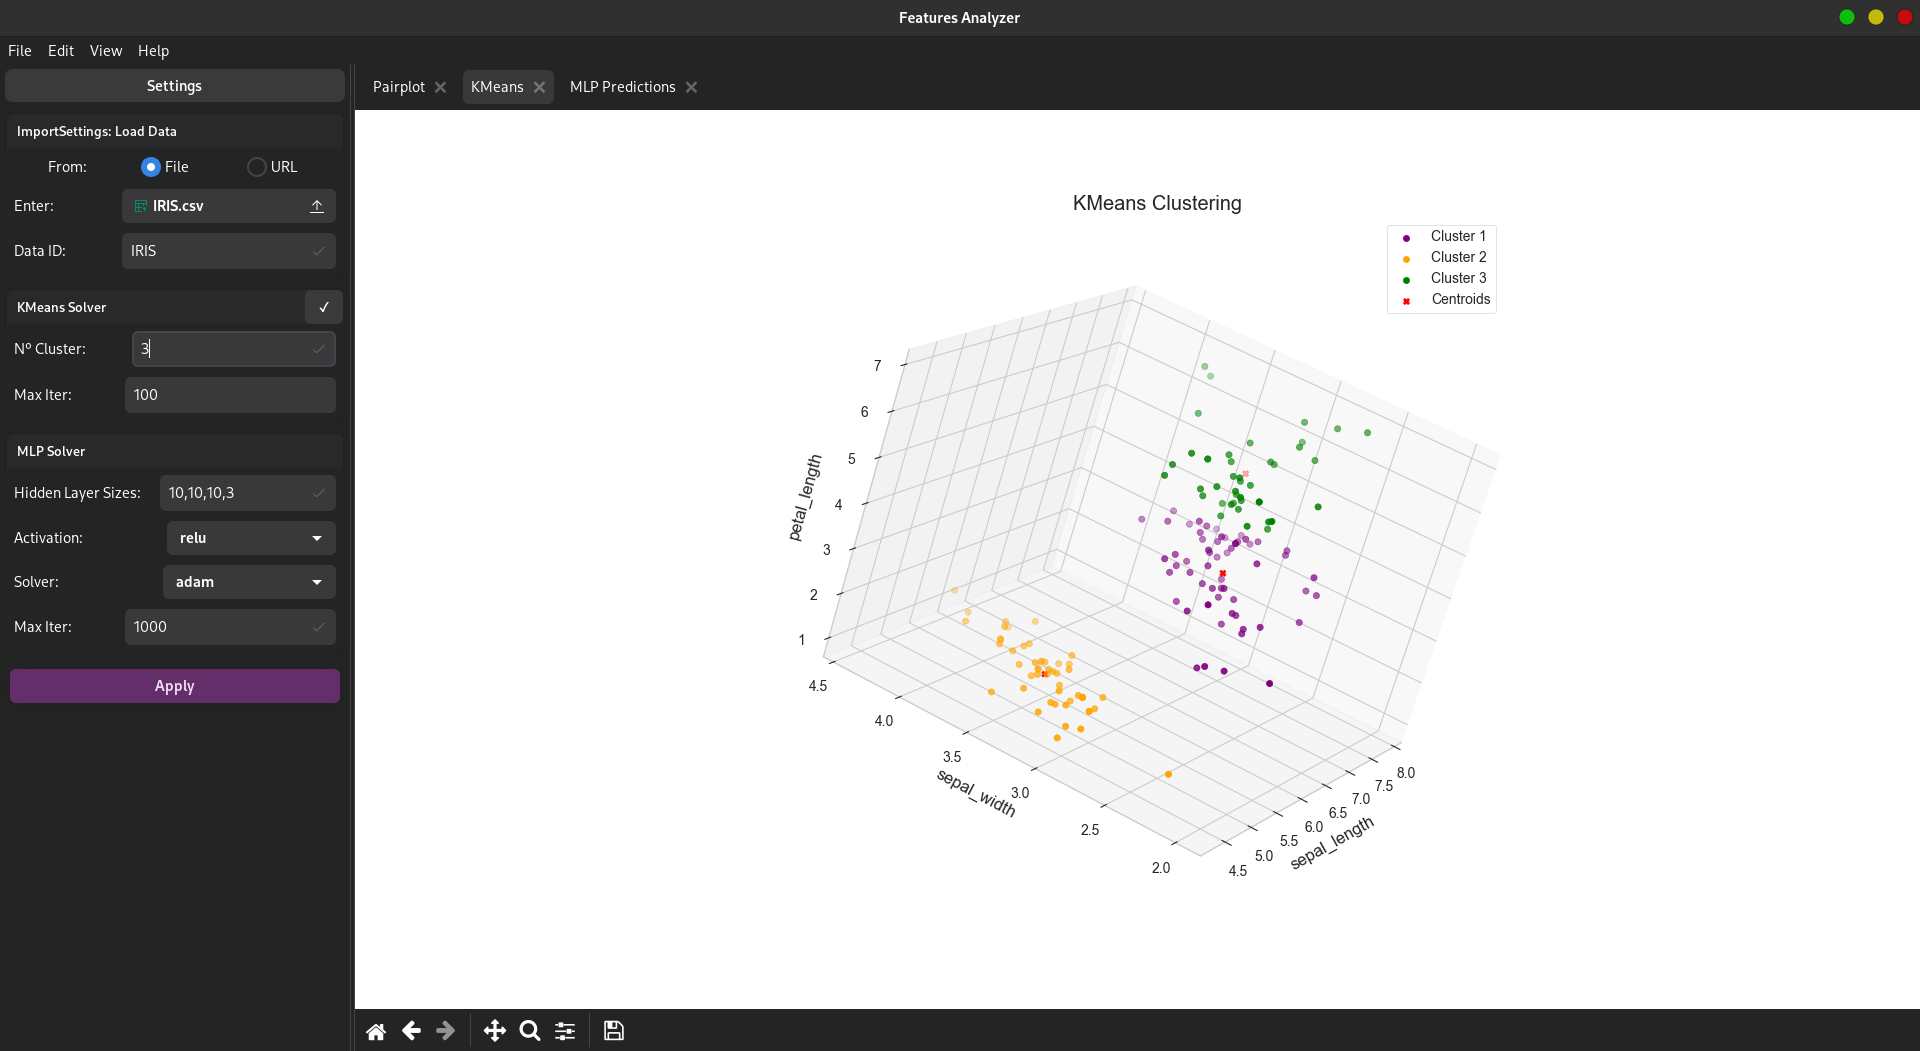
\includegraphics[width=0.8\columnwidth]{image/source/gui.png}}
    \caption{Interface Gráfica do \textit{Boilerplate}}
    \centerline{\textbf{Fonte:} O Próprio Autor (2025)}
    \label{fig:3:gui}
\end{figure}

\begin{itemize}
    \item \textbf{Barra de Ferramentas}: Localizada na parte superior da janela, a barra de ferramentas contém botões para ações comuns, como abrir, salvar e executar, além de menus para configurações e ajuda. Esse componente deve ser ajustado para atender às necessidades específicas de cada aplicação.
    \item \textbf{Barra Lateral} (\textit{sidebar}): À esquerda da janela, a barra lateral exibe os componentes disponíveis para interação, como configurações de importação e parâmetros de modelos. A responsabilidade pela importação dos dados para a memória é gerenciada pela biblioteca \texttt{Pandas}.
    \item \textbf{Área de Trabalho}: O espaço central da janela é dedicado à exibição de gráficos. O componente consiste em um \textit{widget} de \texttt{Gtk.Notebook} que permite alternar entre diferentes visualizações.
\end{itemize}

A interface gráfica é completamente customizável e extensível, permitindo a adição de novos componentes, personalização de estilos e integração com outras bibliotecas gráficas.

A arquitetura do \textit{boilerplate} facilita a criação de interfaces intuitivas e eficientes, oferecendo como exemplo a implementação do \texttt{KMeans} e \texttt{MLP} (\textit{Multi-Layer Perceptron} ou Perceptron de Múltiplas Camadas) para tratar o famoso conjunto de dados flor Iris.

% ========================================================================= %

\section{Utilitários}
\label{sec:3:utils}

\newcommand\urlGhPages{https://docs.github.com/en/pages}
\newcommand\URLGhActions{https://docs.github.com/en/actions}
\newcommand\urlMkdocs{https://www.mkdocs.org/}
\newcommand\urlRuff{https://docs.astral.sh/ruff/}
\newcommand\urlIEign{https://pypi.org/project/python-i18n/}

Nessa seção é apresentado os utilitários desenvolvidos para facilitar a implementação e o uso do sistema. Eles são responsáveis por simplificar a execução de tarefas comuns, como a auditoria do sistema, documentação, análise e formatação, tradução e internacionalização, etc.

\subsection{Logger}

Devido ao grande número de operações e a complexidade da aplicação, surgiu a necessidade de um \textit{logger}, uma ferramenta de uso genérico para auditoria. Ela é responsável por registrar informações sobre o funcionamento do sistema, tanto no terminal de execução atual quanto em um arquivo de log dedicado. Essa funcionalidade facilita a auditoria, depuração e monitoramento da aplicação.

Os logs gerados pelo \texttt{logger} são categorizados em diferentes níveis, cada um com uma cor associada para facilitar a identificação no terminal:

\begin{itemize}
    \item \textbf{\textcolor{blue}{DEBUG}}: Informações detalhadas para diagnóstico. Representado na cor azul.
    \item \textbf{\textcolor{gray}{INFO}}: Informações gerais sobre o funcionamento da aplicação. Representado na cor cinza.
    \item \textbf{\textcolor{ForestGreen}{SUCCESS}}: Mensagens que indicam operações bem-sucedidas. Representado na cor verde.
    \item \textbf{\textcolor{Goldenrod}{WARNING}}: Alerta sobre situações que podem exigir atenção, mas que não são erros. Representado na cor amarela.
    \item \textbf{\textcolor{red}{ERROR}}: Mensagens que indicam falhas que impedem a execução de uma funcionalidade. Representado na cor vermelha.
    \item \textbf{\textcolor{magenta}{CRITICAL}}: Erros graves que requerem atenção imediata. Representado na cor magenta.
\end{itemize}

Os logs são utilizados em vários pontos da aplicação, como na inicialização do sistema, na restauração dos estados, treinamento de modelos e persistência de dados. No trecho a seguir~\ref{lst:logger} é apresentado alguns exemplos simples do uso do \texttt{logger}.

\begin{center}
    \begin{lstlisting}[language=Python, basicstyle=\tiny, caption={Exemplos de uso do \texttt{logger}}, label={lst:logger}]
        logger.info(f"{PREFIX} State dumped.")
        logger.info(f"{PREFIX} State loaded.")
        logger.success(f"{self.__PREFIX} - Model loaded from {self.file_name}.")
        logger.info(f"{self.__PREFIX} - Model binary not found.")
        logger.info(f"{self.__PREFIX} - Model entry not found.")
        logger.error(f"{self.__PREFIX} - {e}")
        logger.warning(f"{self.LOG_PREFIX} Document with UID {uid} not found")
    \end{lstlisting}
    \centerline{\textbf{Fonte:} O Próprio Autor (2025)}
\end{center}

\subsection{Documentação}

A documentação desempenha um papel essencial na manutenção e na extensibilidade de sistemas complexos, como o desenvolvido neste trabalho. Para garantir que os desenvolvedores possam facilmente personalizar e compreender o funcionamento do sistema, foi adotada uma estratégia baseada em \textbf{Markdown} com o uso das ferramentas \href{\urlMkdocs}{\texttt{MKDocs}}\footnote{\url{\urlMkdocs}} e \texttt{mkdocs-material}. Essa abordagem simplifica a criação de uma documentação rica e interativa, que pode ser disponibilizada em formato de site.

A implementação do sistema inclui um gerador automatizado que converte arquivos \texttt{.md} em páginas HTML, CSS e JavaScript estilizadas com o tema \texttt{mkdocs-material}. O resultado é um site responsivo e bem estruturado, armazenado em uma \textit{branch} \texttt{gh-pages} do repositório no GitHub.

Essa \textit{branch} serve como base para a publicação automática do site, tornando a documentação acessível para toda a equipe. As configurações do \texttt{MKDocs} são definidas no arquivo \texttt{mkdocs.yml}, onde é possível personalizar o tema, a navegação, \textit{plugins} e outros aspectos.

\subsubsection{Workflow e CI/CD}

Para automatizar o processo de geração e \textit{deploy} da documentação, foi configurado um \textbf{workflow} utilizando os recursos de integração contínua (CI) e entrega contínua (CD) disponíveis no GitHub. Um \textbf{workflow} consiste em um conjunto de etapas definidas em um arquivo \texttt{YAML}, armazenado no diretório \texttt{.github/workflows} do repositório. Ele descreve os gatilhos (como \textit{commit's}, \textit{pull requests} ou \textit{tags}) e as ações que devem ser executadas, como a instalação de dependências, a execução de testes e a implantação.

O conceito de \textbf{CI/CD} (Integração Contínua e Entrega Contínua) refere-se a práticas que permitem o desenvolvimento, o teste e a implantação de software de forma automática e iterativa. Na integração contínua, alterações no código são frequentemente integradas ao repositório principal, garantindo que ele esteja sempre atualizado e testado. Na entrega contínua, essas alterações são automaticamente implantadas em ambientes de produção ou \textit{staging}, facilitando a liberação de novas funcionalidades.

No caso do gerador de documentação, o workflow configurado no GitHub executa as seguintes etapas:

\begin {enumerate}
    \item \textbf{Gatilho}: O processo é iniciado após um \textit{push} na branch principal do repositório.
    \item \textbf{Configuração do Ambiente}: As dependências necessárias para o \texttt{MKDocs} e o tema \texttt{mkdocs-material} são instaladas.
    \item \textbf{Geração do Site}: O conteúdo em Markdown é processado e convertido em páginas HTML estilizadas.
    \item \textbf{\textit{Deploy} Automatizado}: O site gerado é enviado para a branch \texttt{gh-pages}, que serve como base para a publicação no \textbf{GitHub Pages}.
\end {enumerate}

O \textbf{GitHub Pages} permite hospedar sites estáticos diretamente de um repositório no GitHub, sendo uma solução ideal para publicar documentações. Para ativá-lo, acesse as configurações do repositório, selecione a aba \textit{Pages}, configure a \textit{branch} e o diretório onde os arquivos estão armazenados, e salve as alterações.

Após a configuração, o site será publicado em um endereço gerado automaticamente, como \texttt{https://<username>.github.io/<repository>}, tornando a documentação acessível online de forma prática. Mais detalhes podem ser encontrados na \href{\urlGhPages}{\textbf{documentação oficial}}\footnote{\url{\urlGhPages}}.

Essa abordagem automatizada reduz o esforço manual, garante consistência no processo de \textit{deploy} e promove uma documentação atualizada e acessível, essencial para o sucesso de projetos colaborativos. Embora o \textit{workflow} simplifique o processo, ele pode ser feito manualmente sem grandes dificuldades, seguindo a \href{\URLGhActions}{documentação}\footnote{\url{\URLGhActions}}.

Com este utilitário, os desenvolvedores podem escrever a documentação dos próprios experimentos no projeto e hospedá-los na \textit{web} de forma simples.

\subsection{Análise e Formatação de Código}

A \texttt{Ruff} é uma ferramenta moderna de \textit{linting} (análise de código) e formatação de código desenvolvida para Python. Ele é projetado para ser extremamente rápido e oferecer suporte a uma ampla gama de regras e convenções de codificação, garantindo que o código permaneça legível, consistente e aderente às melhores práticas~\cite{ruff-docs}.

Um \textit{linter} é uma ferramenta que analisa o código-fonte em busca de erros, padrões não recomendados e violações de estilo. Já um \textbf{formatter} formata automaticamente o código para que ele siga padrões predefinidos, como indentação, espaçamento e quebras de linha, facilitando a padronização do projeto.

O \textit{Ruff} destaca-se por oferecer suporte a várias regras e convenções de ferramentas amplamente utilizadas, como \texttt{flake8}, \texttt{isort}, \texttt{pylint}, entre outras. Isso permite integrar múltiplas funcionalidades em uma única ferramenta, simplificando o pipeline de desenvolvimento.

As configurações do \textit{Ruff} são definidas no arquivo \texttt{ruff.toml}, onde podem ser especificadas regras habilitadas, exclusões e personalizações. Esse arquivo centralizado torna o gerenciamento de padrões de estilo mais acessível e compartilhável entre diferentes desenvolvedores de um projeto. Para mais informações, a documentação oficial do \href{\urlRuff}{\textit{Ruff}}\footnote{\url{\urlRuff}}.

\subsection{Tradução e Internacionalização (i18n)}

A internacionalização, comumente abreviada como \href{\urlIEign}{\textit{i18n}}\footnote{\url{\urlIEign}}, refere-se ao processo de adaptação de um sistema de \textit{software} para suportar múltiplos idiomas e culturas sem a necessidade de reengenharia. Esse recurso é essencial para aumentar a acessibilidade do sistema, possibilitando que usuários de diferentes regiões utilizem a aplicação em seus idiomas nativos.

Na implementação, a funcionalidade de \textit{i18n} é gerenciada por arquivos de tradução, que mapeiam as chaves do texto para suas correspondentes localizações. Esses arquivos, frequentemente escritos no formato \texttt{JSON} ou \texttt{PO}, permitem que o conteúdo da interface do usuário seja facilmente traduzido e adaptado para diferentes contextos culturais.

Para o gerenciamento e aplicação de traduções, foi utilizada a biblioteca \texttt{python-i18n}. Essa biblioteca fornece uma interface simples e eficiente para carregar arquivos de tradução, selecionar idiomas e interpolar valores dinâmicos em strings traduzidas.

Além disso, ela suporta recursos avançados, como \textit{fallback} de idiomas (uma linguagem padrão, quando não definida), facilitando a construção de sistemas robustos e internacionalizados.

A configuração da \textit{i18n} utiliza ferramentas específicas que detectam o idioma do sistema ou permitem que o usuário selecione sua preferência. Além disso, o sistema foi projetado para facilitar a inclusão de novos idiomas por meio da simples adição de arquivos de tradução e ajustes mínimos no código.

Essa abordagem promove uma maior inclusão e acessibilidade do sistema, permitindo que usuários de diferentes origens e idiomas possam interagir com a aplicação de forma eficaz e intuitiva.

Sendo assim, instâncias desse \textit{boilerplate} podem ser customizadas para incluir suporte a diferentes idiomas, conforme a necessidade do projeto, útil para aplicações desenvolvidas por equipes multilinguísticas. Na Seção ~\ref{sec:3:consideracoes-finais} é apresentado as considerações finais deste capítulo.


% ========================================================================= %

\section{Considerações Finais}
\label{sec:3:consideracoes-finais}

\newcommand\urlKmeansSolver{https://github.com/ZauJulio/FeaturesAnalyzer/blob/test/src/context/states/kmeans\_solver.py}

Neste capítulo, é apresentada as principais abstrações e componentes do framework desenvolvido, incluindo os conceitos de \textit{State/Observer}, \textit{Widget}, \textit{Controller}, \textit{Module}, \textit{Store}, banco de dados e gerenciamento de modelos.

A implementação seguiu princípios de design orientado a objetos, como encapsulamento, polimorfismo e herança, para garantir modularidade, reutilização e manutenibilidade do código. Abaixo, é descrito como cada componente contribui para a arquitetura do sistema e os métodos de implementação e integração adotados.

\begin{enumerate}
    \item \textbf{\texttt{State/Observer}}: Facilita a comunicação entre componentes. O \texttt{State} representa o estado de um componente, enquanto o \texttt{Observer} notifica mudanças de estado aos demais. Esse componente é essencial para a implementação de todas as funcionalidades.

    \item \textbf{\texttt{Store}}: Gerencia e persiste os estados globais da aplicação. Centraliza os estados em um único contexto, simplificando sua manipulação e persistência, além de oferecer suporte ao salvamento em arquivos. Segue o padrão de projeto \textit{Singleton}.

    \item \textbf{\texttt{Widget}}: Interage com o usuário e exibe informações. Cada \texttt{Widget} está associado a um \texttt{State} e é notificado sobre alterações. Parâmetros ajustáveis são representados por \textit{widgets} filhos, como o \texttt{Gtk.Entry}, usado para entradas de texto ou valores numéricos.

    \item \textbf{\texttt{Controller}}: Conecta a interface gráfica ao \texttt{State}, gerenciando exibição, ocultação e conexões entre sinais dos \textit{widgets} e \textit{handlers} para validação e formatação dos valores.

    \item \textbf{\texttt{Module}}: Garante a consistência do estado dentro de cada domínio, propagando alterações conforme necessário. Encapsula a lógica global do estado, interage com outros módulos e componentes e gerencia notificações de mudanças, como \texttt{on\_untrack} e \texttt{on\_commit}.

    \item \textbf{\texttt{Model}}: Gerencia e persiste os modelos de análise de dados. Implementado com base em \textit{schemas} de validação, assegura a integridade dos modelos. Utiliza a classe \texttt{FAModel}, que fornece métodos genéricos como salvar, carregar e identificar modelos. Um exemplo é o uso do \textit{KMeans}.

    \item \textbf{\textit{Handlers} de Estado}: Atualizam a interface gráfica, persistem estados e gerenciam modelos de análise por meio de um ou mais \textit{Models}.
    
    Esses métodos, estáticos na classe derivada de \texttt{State}, centralizam a lógica de domínio. Por exemplo, no estado do modelo \texttt{KMeans}, o \textit{handler} gerencia as mudanças associadas a esse algoritmo. O \href{\urlKmeansSolver}{\underline{arquivo}}\footnote{\url{\urlKmeansSolver}} fornece um exemplo da utilização dos \textit{handlers} com os modelos.
\end{enumerate}

O capítulo destacou as contribuições de cada componente para a arquitetura do sistema, demonstrando como a integração entre eles proporciona uma experiência de usuário consistente e eficiente. Após toda a apresentação, a arquitetura ilustrada na Figura~\ref{fig:3:cd-arch} complementa a visão geral sobre o sistema.

%%%%%%%%%%%%%%%%%%%%%%%%%%%%%%%%%%%%%%%%%%%%%%%%%%%%%%%%%%%%%%%%%%%%%%%%%%%%%
%% FIM CAPÍTULO                                                            %%
%%%%%%%%%%%%%%%%%%%%%%%%%%%%%%%%%%%%%%%%%%%%%%%%%%%%%%%%%%%%%%%%%%%%%%%%%%%%%
